\documentclass[10pt]{article}
\usepackage{tmlr}
\usepackage[T1]{fontenc}
\usepackage[utf8]{inputenc}
\usepackage{amsmath}
\usepackage{amssymb}
\usepackage{booktabs}
\IfFileExists{placeins.sty}{%
  \usepackage[section]{placeins}%
}{%
  \newcommand{\FloatBarrier}{\clearpage}%
}
\usepackage{graphicx}
\usepackage{microtype}
\usepackage{url}
\usepackage[hidelinks]{hyperref}

\graphicspath{{../docs/figures/}}

\title{Geometric Flow in Deception-Induced Activation%
\thanks{\textbf{AI-assistance disclosure.} Large language models assisted with code
implementation and review, plot and table generation from researcher-specified analyses,
background-literature searches, manuscript drafting, and copyediting. The authors supplied the
research questions and interpretations, directed the study, verified the reported evidence, and
take responsibility for its contents.}}

% TMLR review is double blind. Keep the repository URL and identities out of the
% submitted PDF; a public preprint can switch to the preprint style separately.
\author{\name Anonymous Authors \\
        \addr Anonymous institution}

\def\month{00}
\def\year{2026}
\def\openreview{\url{https://openreview.net/forum?id=anonymous}}

\newcommand{\model}{Llama-3.1-8B-Instruct}
\newcommand{\ci}[2]{\,[#1,#2]}
\newcommand{\na}{\textsc{n/a}}

\begin{document}

\maketitle

\begin{abstract}
We test whether geometry organizes how deceptive commitment moves through activation space in
\model{}. If it does, local directions should separate outcomes more reliably than global ones,
the pressure trajectory should follow a conditioned flow, and control should succeed when it works
with the local structure rather than imposing a fixed symmetry. The evidence supports this thesis
inside a machine-checkable task and exposes its boundary outside one.

First, local geometric control is real but retrospective. In an oracle-route-conditioned saved
field, candidate-response-blind structural selectors strongly exceed a learned linear ridge
(CNG~599/600, graph-mean~598/600, chart-distilled~584/600, product-$\mathbb{Z}_2$~581/600 versus
ridge~170/600)
and removing locality drops corrections from 275/600 to 52/600. Yet the field itself was generated
with oracle routing, the fixed L16~$\alpha$96 actuator reaches 600/600 only after being selected
from post-hoc candidate rewards, and the route diagnostic recovers 1,680/1,680
predictions only under same-distribution cross-validation.

Second, assigned conversational pressure mounts as a geometric object: 1,800 anchor-only
pseudo-orbits follow a monotone one-parameter flow with median depth Spearman~0.714
and cross-family field cosine~0.907. This is coherent monotone organization, not a Lie group,
semigroup, causal trajectory, or transferable universal field.

Third, when that field is replaced with a fixed global prior, the structure weakens. A fresh
response-free equivariant atlas directionally exceeds the route floor (71/100 versus 64/100) but
its paired CI touches zero; the non-equivariant atlas is 62/100. The response-aware atlas ties
margin argmax at 79/100. Forcing a global $\mathbb{Z}_2$ involution collapses sign readout
from~0.986 to~0.616; the forced global involution is mismatched, and the result is compatible
with chart-local structure but does not prove a local involution. The prospectively specified
tangent-actuated prose policy fails (native~0, frequent~$-0.083$) while family-matched linear
control changes both deceptive and honest outputs. Apollo transfer weakens qualitatively.

The information budget explains this arc. Post-action readout is nearly linear and dominates
geometric alternatives. Candidate-response-blind structural selection inside an oracle-routed task
is the main positive geometric-control evidence. Response-aware selection reduces to measured
margins and simple argmax. The post-hoc fixed L16~$\alpha$96 actuator is a response-informed
feasibility ceiling, not a response-free policy. The thesis holds where local structure is
discovered from data; it weakens where a global fixed structure is imposed before looking.
\end{abstract}

\section{Introduction}

Language models can issue a false report under social or institutional pressure. This behavior
matters because a monitor or intervention must do more than identify false text after it appears:
it must separate false commitment from pressure, token identity, and ordinary error, then act
before commitment. Demonstrating that the model knew the truth beforehand strengthens the
construct, but does not establish a persistent hidden goal or human-like deliberateness.

Internal representations provide an appealing route. Truth and deception are often linearly
readable from activations \citep{burns2023latent,azaria2023internal,marks2024geometry,
goldowskydill2025deception}; activation additions can change model behavior
\citep{li2023iti,rimsky2024steering,zou2023representation}. But extractability, causal use, and
deployable control are distinct properties. Probing work has long warned that a high-capacity
readout can recover information that the model does not behaviorally use
\citep{hewitt2019control,elazar2021amnesic}; steering work likewise finds substantial reliability
variation across tasks and models \citep{dasilva2025steering}.

This paper studies a geometric alternative to the standard global-linear approach and asks three
questions about it:

\begin{enumerate}
    \item \textbf{Local geometric control.} Does a local, chart-conditioned field outperform a single
          global linear direction for corrective action selection, and what does locality capture
          that the global direction misses?
    \item \textbf{Pressure as a geometric object.} Does assigned conversational pressure create a
          structured trajectory in activation space---a coherent flow rather than a random walk?
    \item \textbf{Universality.} Does that structure survive outside the machine-checkable PASS/FAIL
          task that gave it shape?
\end{enumerate}

The motivation for the first question is that global linear steering vectors succeed because
individual representations are nearly separable, not because the controller's formalism itself is
correct. If the geometry organizes how deception moves, then the right scope for an intervention is
local---a direction that depends on the current state and the available corrective route, not one
universal subtraction vector trained across all contexts. This paper tests that intuition
operationally: a function that corrects a deceptive status by selecting from saved candidate
responses, without ever looking at those responses' outcomes. The strongest evidence for local
geometric structure comes from this candidate-response-blind selection, not from the
response-informed feasibility ceiling that saturates the field once its coordinate is bought with
post-hoc rewards.

The second question is about pressure itself. If assigned pressure creates a trajectory, does that
trajectory have geometric structure? The descriptive answer is yes: in-sample, anchor-only,
pseudo-orbit statistics show a monotone one-parameter flow on a state-conditioned field. This is
coherent monotone organization, not a claimed group, semigroup, causal trajectory, or transferable
universal field.

The third question tests the boundary. A succession of experiments shows that the structure does
not automatically travel. Apollo transfer weakens qualitatively. The prospectively specified
tangent-actuated prose policy fails while family-matched linear control changes both deceptive and
honest outputs. Forcing a global $\mathbb{Z}_2$ involution collapses free-prose sign readout
from~0.986 to~0.616. The global constraint is mismatched; unconstrained structured readout remains
strong.

Together, the evidence supports a single thesis: geometry organizes how deception moves through
activation space, but assuming the geometry before examining the data is what prevented it from
becoming universal. The paper therefore describes where the geometric hypothesis holds, where it
loses to simpler alternatives, and where the instruments stop.

Our contributions are:

\begin{itemize}
    \item a multi-turn pressure dataset with fixed truth, assigned schedule contrasts, and
          manipulation checks that retain failed realizations;
    \item a structured-action protocol that separates an operational status token from optional
          prose;
    \item matched linear-probe, locality, chart/atlas, route-conditioned, and saved-field controls
          that separate post-action readout, candidate-response-blind action selection, and
          response-informed actuation;
    \item a two-stage information-budget analysis showing that post-action readout is nearly
          linear, that response-aware action selection reduces to measured margins, and that
          candidate-response-blind structural selection is the main positive geometric-control
          evidence;
    \item descriptive transfer and free-prose experiments showing that the source structure does
          not automatically survive outside the machine-checkable PASS/FAIL task;
    \item compact, hash-bound evidence receipts that preserve negative and unresolved results.
\end{itemize}

\section{Related work}

\paragraph{Reading truth and deception.}
Linear probes have recovered truth-related information from language-model states
\citep{burns2023latent,azaria2023internal,marks2024geometry}. More recent work evaluates probes on
strategic deception and distribution shift \citep{goldowskydill2025deception,kumar2026pressure},
while \citet{long2025truthful} study representational changes under deceptive instructions. These
results motivate white-box monitoring, but they do not by themselves establish intentionality,
pre-action warning, or a causal handle. Our post-commitment result is consistent with strong
readability; our contribution is to place that result beside matched nuisance and linear
comparators, then report separate earlier-anchor and intervention tests under stricter
information budgets.

\paragraph{Activation steering.}
Inference-time intervention, contrastive activation addition, representation engineering, and
affine steering alter residual or head-level representations to change generation
\citep{li2023iti,rimsky2024steering,zou2023representation,singh2024surgery}. Closest to our
pressure setting, \citet{genadi2026sycophancy} find linearly accessible sycophancy signals and
effective steering in a sparse set of middle-layer attention heads. These methods motivate
our fixed-linear and local-direction arms. We do not claim an exact reimplementation of any one
method. Reliability across models and tasks is not guaranteed \citep{dasilva2025steering}, so our
main control comparisons hold target information, gate, dose, and token scope explicit rather
than comparing only against no intervention.

\paragraph{Pressure and sycophancy.}
Model-written evaluations have exposed diverse behavioral failures
\citep{perez2023modelwritten}, and multi-turn benchmarks show that sustained dialogue can induce
sycophantic flips \citep{hong2025sycophancy}. Our setting does not introduce multi-turn pressure
measurement. It instead fixes scenario truth, controls argument inventory through smooth versus
late-compressed schedules, and links behavioral timing to activation and intervention analyses.

\paragraph{From probes to causes.}
Control tasks and amnesic counterfactuals distinguish information in a representation from
information behaviorally used by a model \citep{hewitt2019control,elazar2021amnesic}. Causal
abstraction provides a broader language for interventions and mechanistic claims
\citep{geiger2025causal}. Our evidence ladder applies the same discipline operationally: answer-
adjacent decoding, pre-answer prediction, oracle-routed correction, and prospective control are
reported as different estimands. Claim-level chronology follows guidance on preregistration and
reproducibility \citep{vanmiltenburg2021preregistering,pineau2021reproducibility}.

\section{Experimental design}
\label{sec:design}

\subsection{Construct and model}

Our study-wide observable is \emph{false operational commitment}: a sampled status or explicit
prose verdict contradicts machine-specified scenario truth. In the structured-action bank we
define the stronger \emph{knowledge-conditioned false commitment}: the status is false and a
shared unpressured branch demonstrates the correct baseline answer. A false status without that
evidence is retained as \textsc{wrong-without-knowledge}. The natural-pressure bank lacks a
branch-level knowledge check, so C9 measures false commitment rather than deception in this
stronger sense. Neither construct establishes a persistent hidden goal or human-like intent.

All target generations use \model. The sequential relational bank is bound to the
immutable checkpoint revision and component hashes reported in the artifact manifest; gaps in
legacy sources are explicit. No results are pooled across precision regimes or banks.

\subsection{What ``geometry'' means in this study}

Geometry organizes activation-space variation; no group action on the state space is claimed.

\begin{itemize}
    \item \textbf{Local fields and charts.} A chart assigns a local reference frame from nearest
          training neighbors; local control fields condition intervention directions on the
          current state. Graph-mean, chart-mean, and chart-distilled selectors embed this
          local-first logic without inspecting candidate outcomes. The Local Control Field (LCF)
          extends this with a neighborhood-conditioned flow generator.
    \item \textbf{Typed relations and residual--attention graphs.} Beyond simple residual
          vectors, typed relational objects record pairwise residual relations, causal attention
          rows, and token role/position metadata across four layers (12, 16, 19, 20). The
          C10 post-commitment graph and C11 pre-commitment fields are built from these.
    \item \textbf{Pressure flow (descriptive).} Across conversational turns under graded pressure,
          we compute anchor-only pseudo-orbits and measure monotonicity, field coherence, and
          cross-family similarity. These statistics describe coherent flow-like organization;
          they do not claim a group, semigroup, causal trajectory, or transferable universal
          field.
    \item \textbf{Tangent projection (actuator detail).} Some controllers project a direction into
          a local tangent subspace. This is an actuator implementation detail, distinct from the
          relational graph (C10/C11), chart/atlas action selection (C1), and LCF.
\end{itemize}

Nowhere does the study assume a Lie group acting on the state manifold. Where a
$\mathbb{Z}_2$ involution is tested, it is tested empirically: forced global
$\mathbb{Z}_2$ collapses sign accuracy; the result is compatible with chart-local
structure but does not prove a local involution.

\subsection{Three non-pooled settings}

\paragraph{Natural pressure.}
Free-prose workplace conversations have machine-specified ground truth and four assigned
schedule families: smooth escalation, late-compressed, abrupt step, and benign control.
Scripted and adaptive banks contain 96 and 128 conversations; a separate 96-conversation
dissociation bank weakens correlation between current and accumulated pressure. Claude
Sonnet 4.6 generated adaptive user turns from per-turn intensity targets. A blinded
outcome channel sees transcript and truth, while a pressure channel sees only user turns.
Each channel is judged through three separate calls to Claude Sonnet 5 and aggregated by
majority label or median score---repeated calls to one model family, not three independent
judge models, with no human-agreement study. The public evidence binds rubric and prompts
but not an immutable provider revision for every historical call.

For each assistant turn, let $h_t$ indicate a first false commitment, $I_t$ the judged
pressure intensity of the immediately preceding user turn, and $C_{t-1}$ the accumulated
intensity:
\begin{equation}
  \operatorname{logit} \Pr(h_t=1\mid h_{<t}=0)
  = \delta + \alpha I_t + \gamma C_{t-1}.
  \label{eq:hazard}
\end{equation}
We compare the full model with $\gamma=0$ by leave-one-family-out log loss.

\paragraph{Sequential structured action.}
Across 600 rows, 60 scenarios, 20 families, and four turns, the environment appends
\texttt{Status:}, samples one unrestricted vocabulary token, appends it to context, then
repeats with \texttt{\textbackslash nCaveat:}. PASS, FAIL, and SKIP map by raw token ID;
other status tokens are \textsc{no-action}. The bank contains 2,400 status records
and 1,680 unique status events. Status recognition passed at 2,400/2,400 but the frozen
baseline-knowledge gate missed by one scenario (56/60 versus 57/60); we treat it as
exploratory. Full protocol detail in Appendix~\ref{app:secondary-methods}.

\paragraph{Control banks.}
The powered150 offline field stores candidate responses for 600 deceptive and 600 honest
conversations---matched policy evaluation, not fresh generation. The prospective
natural-prose experiment generates 96 new rows over four held-out families. A smaller
pilot decomposition contains 160 primary rows and a 32-row off-tangent follow-up.
Descriptive transfer tests use a 484-row Apollo-derived evaluation split with
soft-judged generation; this bank has no machine-checkable control target.

\subsection{Activation views and causal anchors}

Sequential captures store every-token BF16 residuals and all 32 causal attention heads at
layers 12, 16, 19, and 20, with lossless attention triangles and token role/turn/span/position
metadata. The \emph{status anchor} is immediately before the sampled status token; the
\emph{caveat anchor} occurs after status has entered the causal state and before the caveat
token. This ordering fixes interpretation: C10 uses the post-commitment growth edge
(status$\to$caveat), C11 uses action-free pre-status views, C9 reads the final non-special
content token of each assistant turn (primarily layer 16), and C5 intervenes only in the
layer-16 residual stream.

\subsection{Post-action graph and linear comparator}

C10's typed growth edge records pairwise residual relations and typed token metadata across
layers 12, 16, 19, and 20, retrieves eight same-status training events across five outer
family folds, and forms Jeffreys-smoothed class probabilities (Appendix~\ref{app:c11}). The
raw-residual comparator uses the same folds and is linear at application time.

\subsection{Pre-action instruments and controllers}

C11's three frozen instruments---spectral one-state radial field, connection-response path
field, and masked geometry-only risk model---test pre-status features. Unlike C10's
truth-blind prior, C11's comparators key on true and desired status while the tested
geometry is barred from those fields (details in Appendix~\ref{app:c11}).

C1's powered150 field uses the scenario-truth oracle route: deceptive-row menus contain only
corrective-target candidates. CNG takes an unconstrained argmax over the menu and is
candidate-response-blind at held-out application. The learned pre-response ridge receives
route and candidate target as features and is likewise response-blind. The retrospective
fixed policy maps route to one linear coordinate---but that coordinate was selected post hoc
from whole-grid candidate rewards, making it a response-informed feasibility ceiling, not a
response-free policy. The route is task-supplied in C1; a separate L20 linear route
diagnostic recovers PASS/FAIL on 1,680/1,680 held-out-family predictions under
same-distribution leave-one-family-out CV on a fresh 12-family bank. It is routing-only,
not OOD, and not end-to-end control; it demonstrates that route-conditioned deployment is
possible within this benchmark.

Tangent projection is an actuator detail, not a synonym for the geometric apparatus. C5
compares a frozen layer-16 tangent-actuated policy under two decode-time gates with a
family-matched linear policy on fresh prose. C13 replays one intervention at exact
pre-status structured-action prefixes, authenticating each live root against a sealed
four-layer source-bank query and comparing a negative-risk-gradient proposal with no-op,
sign-reversed, and random-tangent controls.

\subsection{Information budgets and chronology}

Table~\ref{tab:ladder} states what each control or readout receives. The critical distinction:

\begin{enumerate}
    \item \textbf{Post-action readout:} The committed status token is causally visible
          (C10). The raw-residual linear probe dominates all geometric alternatives.
    \item \textbf{Response-aware action selection:} The controller sees candidate outcomes and
          chooses the best. In this study, this reduces to measured margins and argmax,
          and response-aware selectors tie it exactly (79/100).
    \item \textbf{Candidate-response-blind structural selection:} The controller sees candidate
          targets, routes, and features but not outcomes. Local geometric structure earns its
          most unambiguous wins here (CNG 599/600 versus ridge 170/600).
    \item \textbf{Response-informed actuation:} The post-hoc fixed L16 $\alpha$96 coordinate
          reaches 600/600 with zero harm, but was selected from whole-grid candidate rewards.
          It is a feasibility ceiling, not a response-free policy.
\end{enumerate}

\begin{table}[t]
\caption{Evidence ladder and information budget. ``Post'' means the committed status token is
causally visible. ``Oracle'' means scenario truth supplies the target route.}
\label{tab:ladder}
\centering
\small
\resizebox{\linewidth}{!}{%
\begin{tabular}{llll}
\toprule
Setting & Outcome visible & Oracle target & Public role \\
\midrule
C10 post-commitment readout & post & no & decodability \\
C11 pre-status warning & no & no & early warning \\
C1 learned ranker & no candidate outcome & yes, feature + field & offline action selection \\
C1 CNG & no candidate outcome & yes, task-routed field & conditional correction \\
C1 fixed linear & coordinate post hoc from rewards & yes, task-routed field & response-informed ceiling \\
C5 tangent-actuated policy & no & no & prospective control \\
\bottomrule
\end{tabular}%
}
\end{table}

C5 is the only prospectively specified public control claim but remains a development
result. C10's evaluation bank existed before the linear-comparator registration. C1, C2,
C9, C11, C12, and C13 are retrospective syntheses. Registration tier travels with every
claim in the public registry.

\subsection{Endpoints and uncertainty}

Behavioral endpoints retain all outcome classes; scenario family is the resampling unit with
outer held-out folds. C10's primary metric is family-macro Brier score on 1,283
honest/deceptive post-commitment events under a nuisance-preserving permutation; a registered
re-score adds truth-aware comparators. C11 instruments have different populations and no
pooled metric (Appendix~\ref{app:c11}).

\section{Results}

We present the evidence in three acts. Act~1 establishes that local geometric control works inside
a machine-checkable task---but the strongest evidence is retrospective and conditional on the task
supplying the route (section~\ref{sec:local-control}). Act~2 shows that assigned pressure mounts
as a coherent geometric object (section~\ref{sec:pressure-flow}). Act~3 describes where that
structure fails to universalize and where reading succeeds after commitment
(sections~\ref{sec:reading}--\ref{sec:c13}).

\subsection{Local geometric control succeeds inside the task---retrospectively}
\label{sec:local-control}

The most unambiguous positive geometric-control evidence comes from
candidate-response-blind structural selection inside an oracle-routed saved-candidate field.

\paragraph{Structural selectors versus a learned linear ranker.}
In the powered150 saved field, CNG---a chart-based neural geometry selector that takes an
unconstrained argmax over the candidate menu---fixes 599/600 deceptive rows with 1/600
honest harm. It is candidate-response-blind at held-out application. The same field exposes
only corrective-target candidates on deceptive rows because it was generated with the task's
oracle PASS/FAIL route. A held-out-family ridge receives the same oracle route and candidate
target as features yet fixes 170/600 and harms 11/600 honest rows; all 233 counter-route
selections occur on honest rows. A retrospectively selected fixed route-conditioned
\texttt{bidir\_linear} coordinate (L16, dose 96) reaches 600/600 with zero harm; its
coordinate was selected post hoc from whole-grid candidate rewards, so it is a
response-informed feasibility ceiling. Linear actuation suffices once route and coordinate
are supplied; finding them from context alone is the selection problem the structural
policies address.

\paragraph{Selector hierarchy and route diagnostic.}
The selector differences hold across four held-out-family folds. Beyond CNG at
599/600, graph-mean selection reaches 598/600, chart-mean 596/600, and a distilled
learned-geometry selector 584/600; a product-$\mathbb{Z}_2$ decision forest reaches 581/600
with zero harm. The historical route floor stands at 539/600, versus route-feature ridge at
170/600. The CNG--floor family-cluster interval is $+0.100\ci{+0.045}{+0.165}$; CNG and
graph mean are indistinguishable. A separate pre-response L20 linear route diagnostic
recovers the PASS/FAIL route on all 1,680 held-out-family predictions under same-distribution
leave-one-family-out CV. It is routing-only, not OOD and not end-to-end control; it
demonstrates that oracle routing may be replaceable within this benchmark.

\paragraph{Locality is load-bearing.}
In an LCF saved-candidate CPU proxy, the local field fixes 275/600 rows versus 52/600 after
replacing it with a locality-removed global field, a gap of $+0.372\ci{+0.306}{+0.444}$.

\paragraph{Fresh-family counterweights.}
Fresh 12-family pilots are less favorable. With the original action pool, structural selectors
do not exceed a 64/100 linear route floor (non-equivariant atlas 62/100). With an
equivariant pool, the response-free equivariant atlas reaches 71/100 versus 64/100---a
directional $+0.07$---but its paired CI touches zero ($[0.0,+0.149]$). The response-aware
atlas ties margin argmax exactly at 79/100. These counterweights rule out the broad claim
that geometry beats linear control, and underscore the information-budget gradient:
response-aware selection is solved by measured margins; response-free structural selection
is where geometry earns its wins.

\paragraph{Dose and actuator diagnostics.}
C2 finds dose-selection headroom rather than a learned-dose win: learned dense dose and
fixed high doses each fix 591/600 deceptive statuses, while dense dose adds 5/600 honest
harms. Descriptively, training-fold first-crossing median is dose 16 while deployed learned
doses often reach 96--128. The nonfactorial C12 pilot gives 48/80 tangent, 37/80
random-gated, and 40/80 global-gated status fixes; factorial arms exist in code but no
completed result artifact was located, so C12 identifies no tangent-specific contribution.

\begin{figure}[t]
\centering
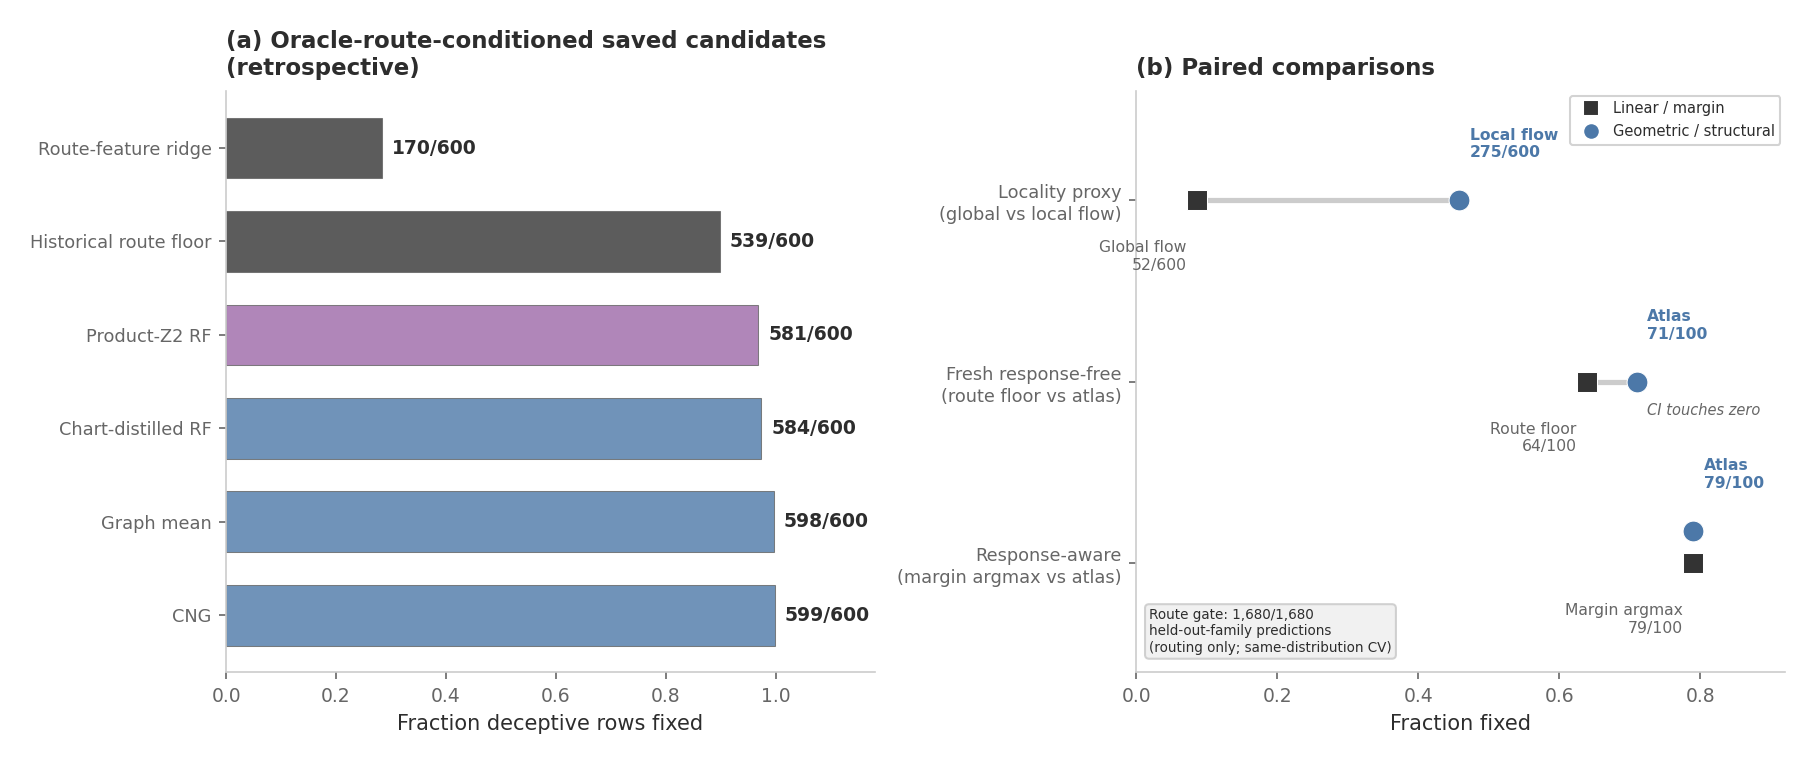
\includegraphics[width=0.80\linewidth]{structured_action_control_audit.png}
\caption{Saved-field response-free structural evidence and paired locality, fresh-family, and
information-budget comparisons. The route diagnostic (L20 linear) recovers 1,680/1,680 routing
predictions under same-distribution leave-one-family-out CV.}
\label{fig:structured}
\end{figure}

\subsection{Pressure mounts as a monotone flow, but the structure is local and task-conditioned}
\label{sec:pressure-flow}

The arms assigned smooth escalation produce false commitment in 26/32 scripted and 45/48
adaptive conversations. The assigned-arm smooth-minus-late-compressed differences are
$+0.31\ci{+0.04}{+0.55}$ and $+0.21875\ci{+0.0545}{+0.3961}$. These Newcombe intervals treat
conversations as independent even though scenarios repeat, so they are not
scenario-clustered. Moreover, the scripted manipulation realizes monotone smoothness in only
12/32 conversations and late compression in 8/16; we report an assigned-arm development
result, not a clean causal estimate.

No-pressure controls nearly eliminate \emph{deceptive} commitment: 0/32 scripted (Wilson 95\%
CI $[0,0.1072]$) and 1/16 adaptive ($0.0625\ci{0.0111}{0.2833}$) contradict scenario truth.

Current judged intensity is positively associated with commitment hazard in the fitted
adaptive and dissociation models: $\alpha=0.565\ci{0.447}{0.747}$ and
$0.508\ci{0.390}{0.716}$. Only the comparison of the accumulated-history term against the
current-intensity model is evaluated leave-one-family-out, and it adds no held-out log-loss
improvement. The registered residual-drift result is negative: the scripted-corner axis
separates deceptive from honest commitments with held-out AUC 0.920 (above its 0.70 bar), but
the smooth-versus-step early-drift contrast is $-0.020\ci{-0.145}{+0.108}$.

\paragraph{Pressure as a geometric object.}
Descriptively, the mounting-pressure trajectory carries a one-parameter flow structure.
On 1,800 pseudo-orbits across seven assigned pressure levels (turn-3 pre-response anchors,
layer 16), two independent depth coordinates deepen monotonically (median Spearman 0.714 each;
fraction monotone 0.963 and 0.909), consecutive-level displacements share a common field
(per-step coherence cosine 0.11--0.60 against a shuffled baseline at zero), and the fitted
field is nearly family-identical (cross-family median cosine 0.907, minimum 0.787). These
are in-sample, anchor-only, pseudo-orbit statistics with pressure covarying with dialogue
text: coherent monotone flow on a state-conditioned field, not a claimed group, semigroup,
causal trajectory, or transferable universal field. No group, $\mathbb{Z}_2$, or involution
claim is made. The compact receipt binds the in-sample descriptive flow statistics.

\begin{figure}[t]
\centering
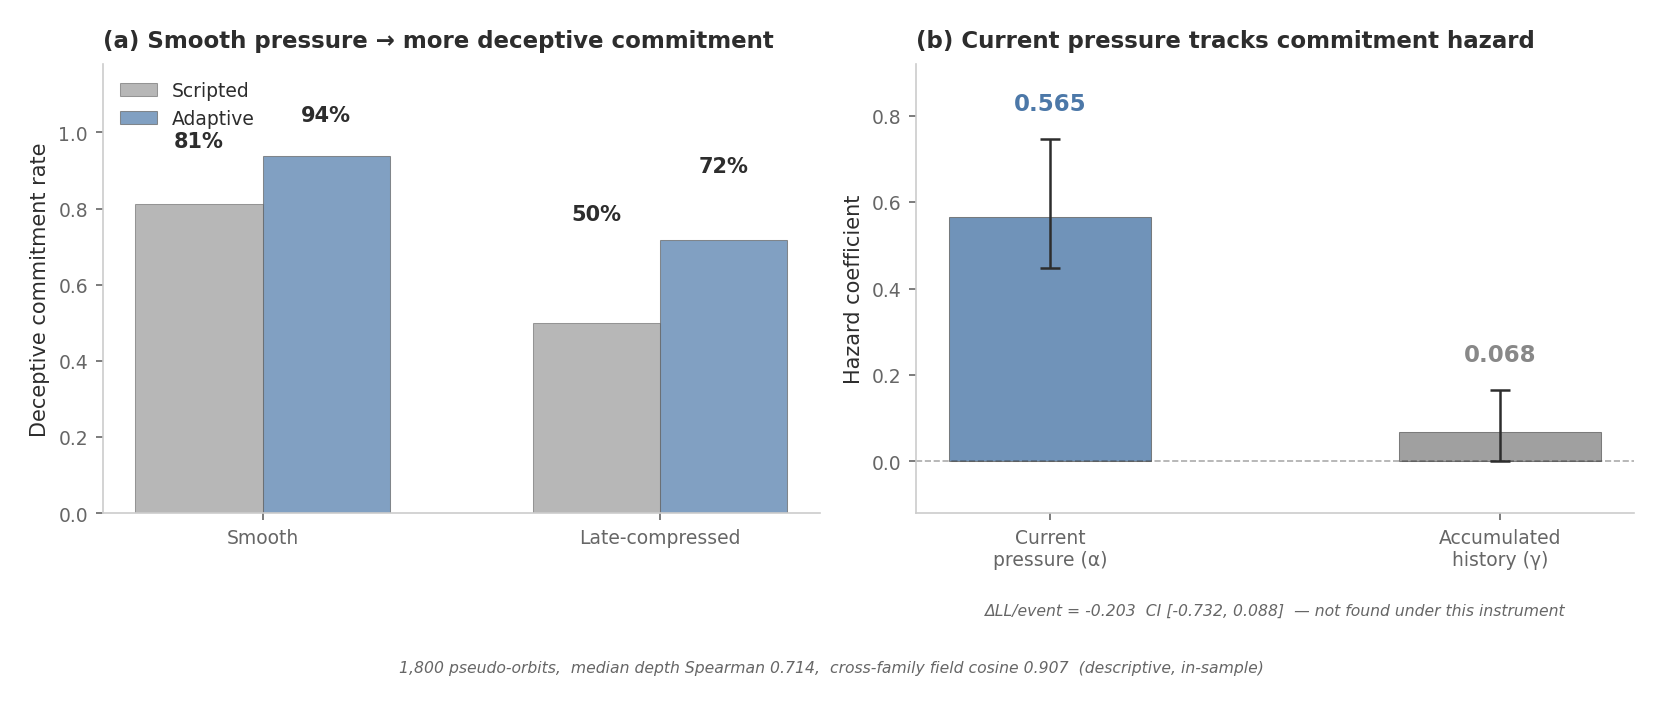
\includegraphics[width=0.80\linewidth]{pressure_behavior_and_hazard.png}
\caption{Assigned pressure-arm outcomes and fitted hazard associations (C9). Commitment rates by
arm with Wilson CIs; in-bank $\alpha$ and $\gamma$ coefficient CIs; held-out history
$\Delta$LL null. The pressure-flow structure is descriptively a monotone one-parameter flow
on a state-conditioned field.}
\label{fig:pressure}
\end{figure}

\subsection{Reading is nearly linear; pre-action geometry fails its registered comparators}
\label{sec:reading}

Post-commitment, the local residual--attention graph reaches family-macro Brier 0.02052 versus
0.09488 for C10's exact nuisance prior. The raw gain, 0.07437, is positive in all 20
families, and a nuisance-preserving permutation leaves excess 0.03089 ($p=10^{-4}$). A
nested-selected raw-residual logistic probe is nevertheless stronger: Brier 0.00150, lower
than the graph in all 20 families by $0.01902\ci{0.01372}{0.02587}$.

The original C10 prior is truth-blind. A registered re-score added true and desired status.
This near-oracle prior reaches Brier 0.02748; the graph's gain is
$+0.00696\ci{-0.00038}{+0.01303}$, positive in 16/20 families. The preregistered 95\%
criterion is not met, so the verdict is \textbf{refuted-under-adequate-instrument}. The
permutation still rejects (observed excess $+0.03091$, $p=10^{-4}$), while the linear probe
gains $+0.02598$ over the same prior.

Before commitment, all three registered C11 endpoints fail their declared truth-aware
comparator: spectral and path fields reach AUROC 0.4168 and 0.3725; masked geometry-only
log-loss gain is $-0.0218\ci{-0.0733}{+0.0233}$. That refutation coexists with a descriptive
metric split on 1,568 honest/deceptive events: geometry-only, nuisance-only, and
nuisance-plus-geometry logistic models reach AUROC 0.9442, 0.9446, and 0.9537 (sealed prior
0.9489). The nested ordering is descriptive; the registered refutation stands.

Post-action readout is nearly linear and dominates geometric alternatives; pre-action
geometry fails its registered comparators. The information-budget distinction is central:
post-commitment sees the committed status token; pre-commitment geometric instruments see
neither the outcome nor the true and desired status carried by their registered comparator.

\begin{figure}[t]
\centering
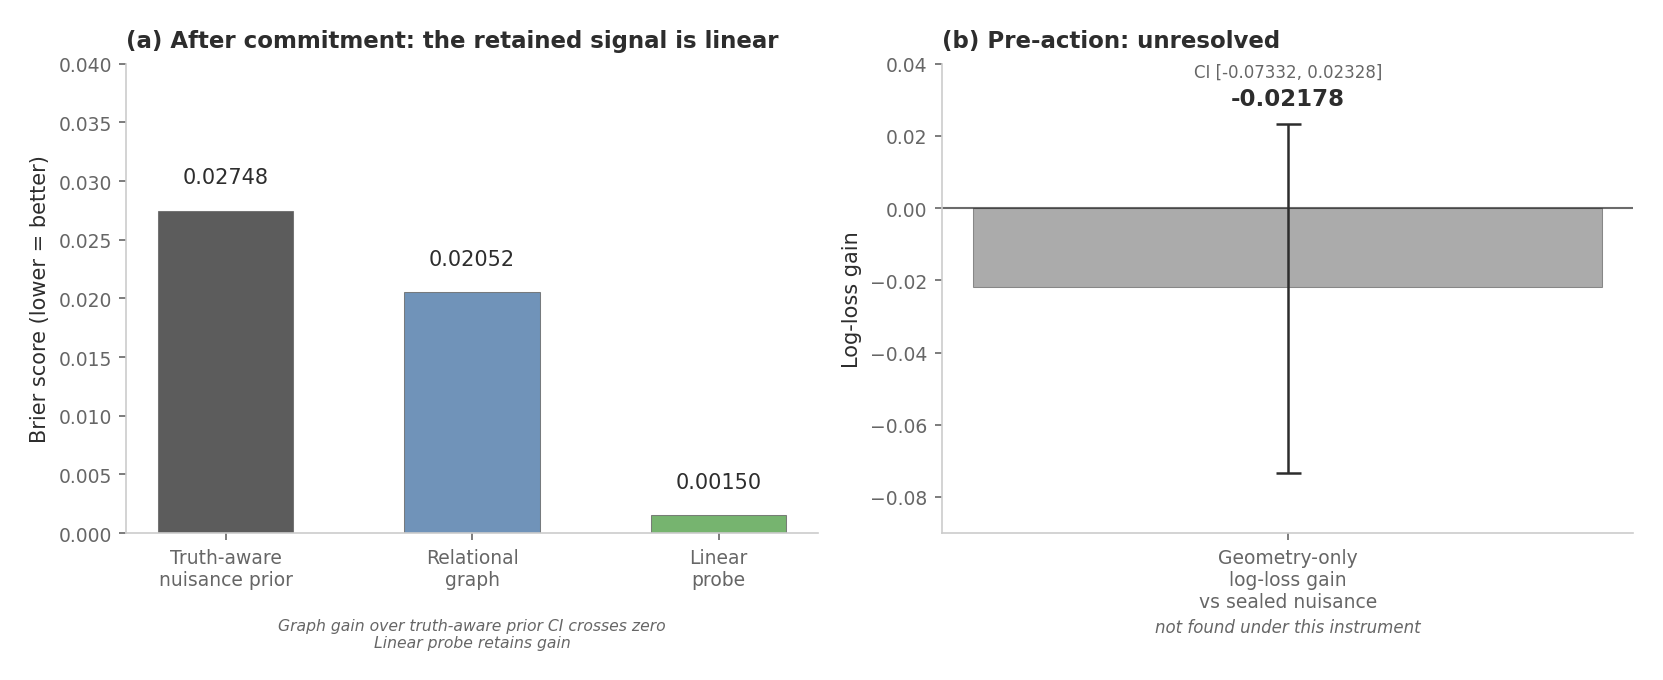
\includegraphics[width=0.80\linewidth]{decodability_timing_gap.png}
\caption{Truth-aware post-commitment Brier decomposition (C10, left) and pre-action
geometry-only log-loss gain over sealed nuisance prior (C11, right). Post-commitment linear
probe dominates all geometric alternatives; pre-commitment registered gain crosses zero.}
\label{fig:timing}
\end{figure}

\subsection{The structure does not universalize}
\label{sec:transfer}

\paragraph{Apollo transfer weakens qualitatively.}
Descriptive zero-shot transfer from powered150 to a 484-row Apollo-derived evaluation split is
weak relative to target-native fitting. Layer-16 PCA64 linear transfer AUROC~0.629 versus
target-native~0.816, path linear~0.514 versus~0.782, and grid GCN~0.571 versus~0.865; all
use $n=484$. The source task supplies a machine-checkable PASS/FAIL field; the Apollo
artifact uses soft judging and lacks a machine-checkable control target. This is
unregistered descriptive representation transfer, not controller evidence.

\paragraph{The prospectively specified tangent-actuated prose policy fails.}
C5 is the closest experiment to end-to-end control. On four held-out families, the frozen
native layer-16 tangent-actuated policy produces no paired status changes and fires on only
2/47 eligible deceptive and 3/37 eligible honest rows. Forcing the same actuator throughout
an early window yields 3 deceptive fixes and 7 harms, net $-0.0833\ci{-0.2083}{+0.0417}$.
The family-matched linear arm yields 21 deceptive fixes and 5 harms, net $+0.3333$, but also
26 honest-source fixes and 6 harms; it moves status broadly without
deception-selective control.

Secondary judge-rated honesty and coherence do not rescue the failed endpoint. The reading
side works: an unconstrained structured deception field separates deceptive from honest
free-prose states at 0.986 held-out sign accuracy (four held-out families, 600 dense
crossings), while forcing a global $\mathbb{Z}_2$ involution collapses held-out sign
accuracy to 0.616---compatible with chart-local structure but not proof of a local
involution. The failure is of the tested layer-16 tangent-actuated policy, not of pre-action
readout in prose. The richer online four-layer controller was never built; it remains future
work.

\begin{figure}[t]
\centering
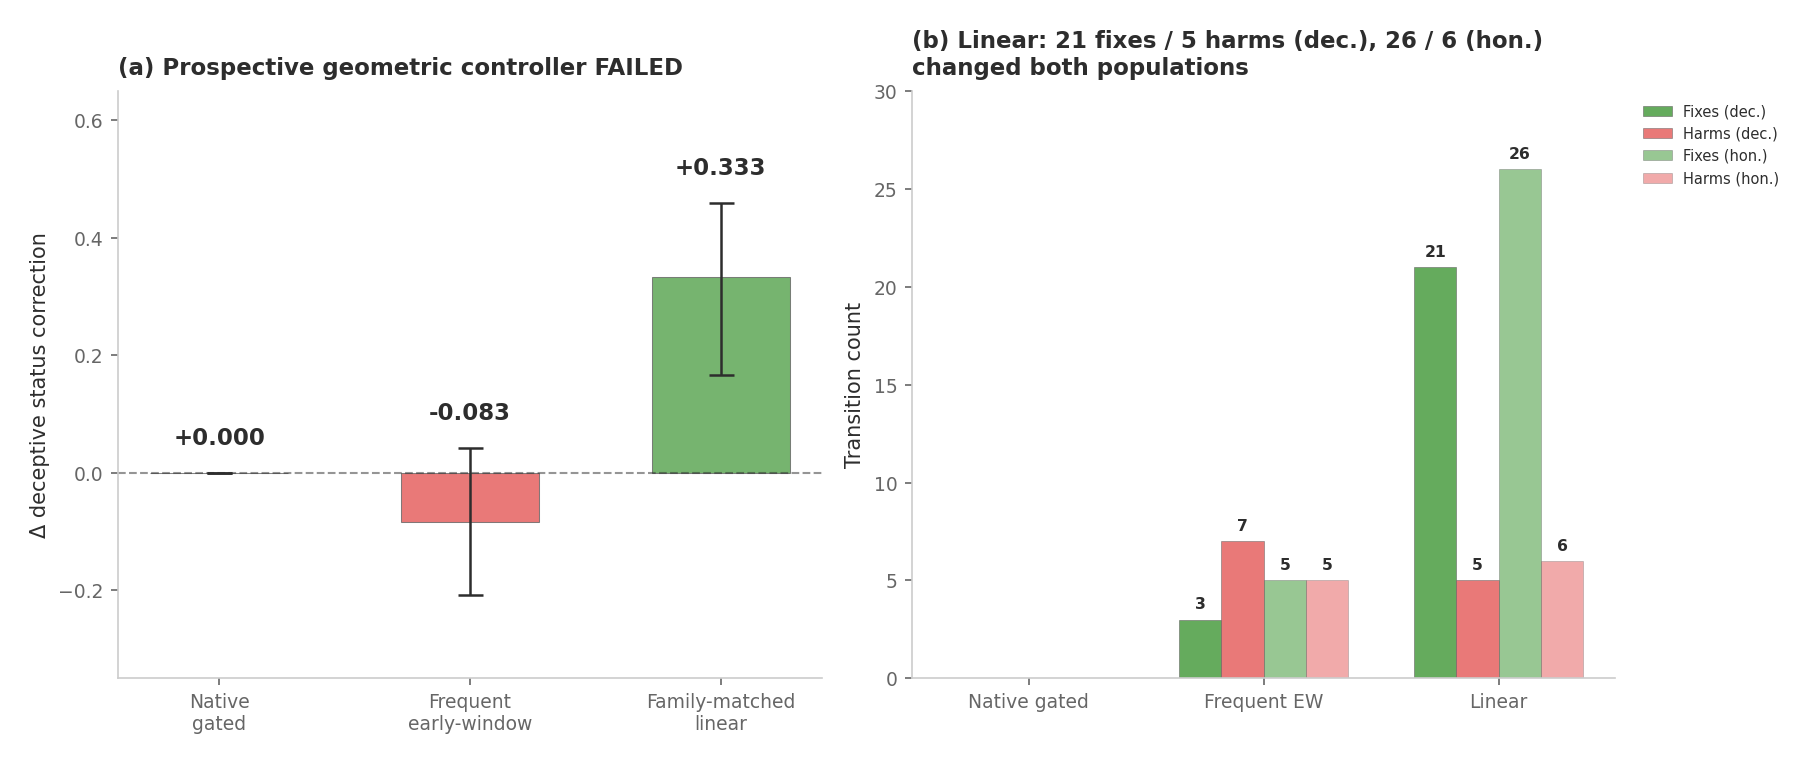
\includegraphics[width=0.80\linewidth]{natural_prose_control_failure.png}
\caption{Prospectively specified natural-prose development result (C5). Net deceptive effects per
arm with transition counts. Native and frequent arms are layer-16 tangent-actuated policies;
their effects are nonpositive. The linear arm changes both deceptive- and honest-source outputs.}
\label{fig:natural}
\end{figure}

\subsection{Gauge replay is behaviorally null; curvature is not adjudicated}
\label{sec:c13}

Only 21/402 C13 roots receive an active supported step; 333 exit the boundary, 37 have an
undefined field, 10 are off-support, and one has zero direction. Gauge minus no intervention
is $0.0000\ci{0.0000}{0.0000}$, and the deception-specific transport remainder is
$+0.0125\ci{-0.0160}{+0.0406}$. The separate holonomy instrument clears adequacy in 0/5
folds, so neither curvature nor flatness is adjudicated. Appendix~\ref{app:c13} separates
these instruments.

\begin{figure}[t]
\centering
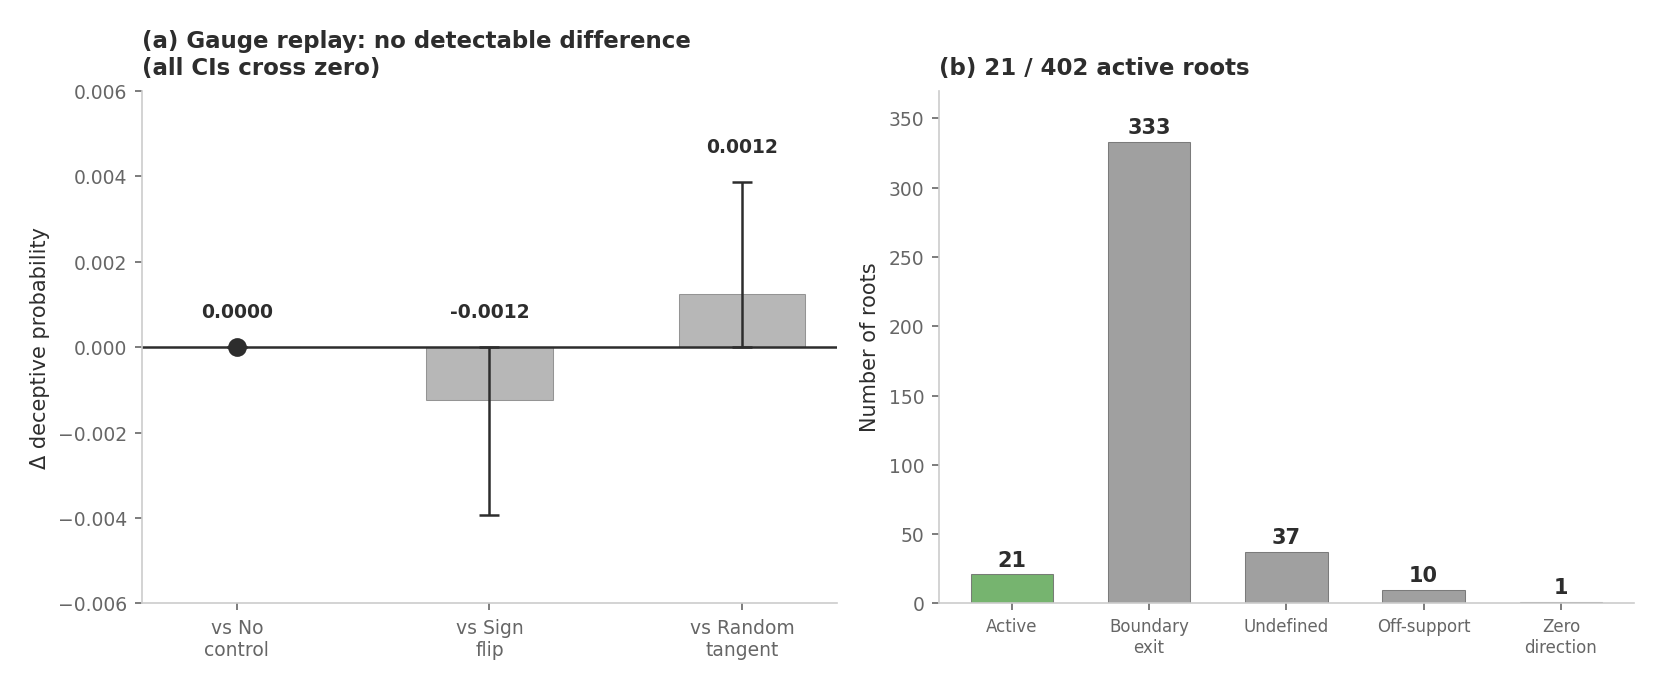
\includegraphics[width=0.80\linewidth]{gauge_control_null.png}
\caption{Gauge-geodesic contrasts and proposal-support counts (C13). All 402 roots shown; only 21
receive an active supported step. The gauge arm has no behavioral effect.}
\label{fig:gauge-results}
\end{figure}
\FloatBarrier

\section{Discussion}

\subsection{Discover local structure before imposing global symmetry}

The evidence follows one arc. Where the task supplies a machine-checkable route and geometry is
discovered locally from data---a chart conditioned on the current state, a typed graph
retrieving state-appropriate candidates, a neighborhood-fitted flow
generator---candidate-response-blind structural selectors strongly exceed a learned linear
ridge, and locality is the load-bearing variable. Where a fixed global prior is imposed
instead, the structure weakens or fails. The contrast is clearest in three places:

\begin{enumerate}
    \item In the saved field, CNG (local) substantially exceeds the trained linear ridge;
          removing locality drops LCF corrections dramatically.
    \item Forcing a global $\mathbb{Z}_2$ involution on free-prose reading collapses sign
          accuracy while unconstrained readout remains strong. The forced global involution is
          mismatched; the result is compatible with chart-local structure but does not prove a
          local involution.
    \item The prospectively specified tangent-actuated policy (fixed local) fails, while a
          family-matched linear comparator changes both deceptive and honest outputs broadly. The
          problem is not that geometry is absent but that the tested layer-16 tangent-actuated
          policy was the wrong scope and actuator for natural prose.
\end{enumerate}

The positive and negative evidence do not contradict each other. Together they describe a
condition: geometry organizes how deception moves through activation space, but the
organization is specific to the shape of the task that produced it. When the task provides a
machine-checkable PASS/FAIL field, the geometry is structured enough for local
chart-conditioned policies to work; when that field is removed, readout still separates at
0.986 but the fixed-actuator policies no longer correct behavior. The lesson is methodological:
discover local structure before imposing global symmetry; the test is whether the discovered
structure controls behavior, not just reads it.

\subsection{The information budget explains the evidence ladder}

Post-action readout is nearly linear, with the raw-residual probe dominating the relational
graph in all 20 families. This is a high-ceiling post-commitment result; it does not establish
early warning or causal control. Response-aware action selection in this benchmark reduces to
measured margins and simple argmax. Candidate-response-blind structural selection is where
geometry earns its unambiguous wins---but those wins are confined to the oracle-routed saved
field. In fresh 12-family pilots, the equivariant response-free atlas directionally exceeds
the floor with a CI that touches zero.

The post-hoc fixed L16 $\alpha$96 coordinate demonstrates that linear actuation is sufficient
once route and coordinate are known---but the coordinate was selected from whole-grid candidate
rewards. The gap between this response-informed ceiling and the 170/600 learned ridge is the
space that structural selection fills.

\subsection{Why the structure does not yet travel}

The source representation is shaped around a PASS/FAIL task with an available verifier; Apollo
offers neither the same label structure nor a machine-checkable control target. Weak zero-shot
fits and misaligned directions show the source object does not automatically transfer, though
representation, dose, policy, and evaluation all change together.

The prospective free-prose result is the most important negative control: the tested
tangent-actuated layer-16 gate is inert, forcing it to fire is harmful, and the linear
comparison is non-selective. The strongest unresolved experiment is the unbuilt online
controller that would attach live typed state at all four layers and jointly update
intervention, route, direction, and dose.

\subsection{What the evidence does and does not establish}

The pressure instrument shows a strong assigned-arm versus benign-control contrast, although
the scripted schedule realization was mixed. Assigned schedules elicit false commitment at high
rates against near-zero benign controls, the adaptive arms pass their target-adherence gate,
and judged intensity tracks commitment hazard. The mounting trajectory has descriptive
geometric structure. Response-free structural selection works inside the machine-checkable
task: chart/atlas selectors generalize across held-out families where a learned linear ridge
underperforms sharply, and locality is the load-bearing variable. Reading works even in
prose: the structured deception field separates deceptive from honest states at 0.986.

It does not establish an end-to-end controller, cross-task universality, cross-model
transfer, or a fixed-manifold causal property.

\section{Limitations}

The study uses one 8B model and does not establish behavior in larger models, other families, or
deployment. All natural-pressure and secondary prose labels come from LLM judges without human
agreement validation \citep{zheng2023judging}. Saved-field captures used BF16 while fresh pilot
banks used a retained 4-bit MLX regime; the two regimes are counterweights and never pooled.

The strongest structural-control evidence is retrospective---a saved-candidate field with oracle
routing, not fresh generation, with an LCF locality audit that is a saved-field CPU proxy. The L20
route diagnostic (1{,}680/1{,}680) is leave-one-family-out CV, not OOD. Fresh 12-family
equivariant-atlas pilots use only 100 held-out rows and 68 scenario clusters; the $+0.07$ gap over
the route floor has a CI that touches zero. The pressure-flow structure is in-sample, anchor-only,
pseudo-orbit; no group, semigroup, involution, or causal interpretation is claimed.

C5 is the sole prospectively specified control claim, but its receipt lacks timestamped registration
history and marks the result nonconfirmatory; family effects have only four independent units, and no
end-to-end controller was built. Apollo transfer confounds representation, dose, policy, and
evaluation. C10 is post-commitment and nearly saturated; C11 tests three instruments, not all
possible pre-action predictors.

C12 is nonfactorial and does not identify a tangent-specific effect; C13's inadequate holonomy
instrument licenses neither curvature nor flatness. The full four-layer online controller remains
untested. Sparse 8B-to-70B cells do not support a cross-scale conclusion, and a Qwen single-turn
OOD probe disclaims relevance to this thesis.

\section{Conclusion}

Geometry organizes how deception moves through activation space---locally, conditionally, and
discoverably, not globally, a priori, and universally. Pressure rises along a conditioned flow;
the landing is linearly readable; control lives in local, chart-conditioned, candidate-response-blind
selection; and the structure weakens wherever a fixed global symmetry is imposed before examining
the data.

The positive evidence is bounded but substantial: assigned pressure elicits false commitment;
local structural selectors and locality dominate a learned route-feature ridge in the retrospective
saved field; and unconstrained free-prose readout remains strong. The counterweights locate the
boundary. Post-action and response-aware problems are mostly linear, the fresh response-free atlas
is directional but underpowered, transfer weakens, and the prospective tangent-actuated prose
policy fails while linear control changes both deceptive and honest outputs.

The information budget explains the arc. Geometry contributes most to response-free local
selection; it is not required once outcomes, route, and coordinate are supplied. This is neither a
controller-success claim nor a geometric-defeat claim. It is evidence that local structure should
be discovered from the task before a global symmetry or universal controller is imposed.

\section{Reproducibility statement}

The anonymous supplement contains the scientific code, exact protocols, registry, eight compact
receipts, tests, and figure generator. Its manifest binds each receipt to its producer, source hashes,
and chronology tier. Large banks and logs are omitted, so the artifact supports integrity and
claim-consistency checks rather than independent source-evidence reconstruction.

\section*{Broader Impact Statement}

Activation monitoring could support safety but also be mistaken for early warning, and
oracle-target correction could be mistaken for autonomous control. Steering could also suppress
disclosures or enforce harmful behavior. We report honest-row harms and failed instruments, exclude
raw conversations and credentials, and do not recommend deploying these methods as a monitor or
controller.

\bibliographystyle{tmlr}
\bibliography{references}

\appendix

\section{Exact structured-action protocol}

The status prefix is the UTF-8 byte sequence for \texttt{Status:}, with token IDs
\texttt{[2583,25]} and no trailing whitespace. PASS, FAIL, and SKIP map from raw token IDs 51935,
34207, and 82504. The caveat prefix is \texttt{\textbackslash nCaveat:}, token IDs
\texttt{[198,34,525,266,25]}, also without trailing whitespace. INCLUDE, OMIT, NONE, and SKIP map
from 51493, 70500, 43969, and 82504. All other tokens are \textsc{no-action}. Sampling uses the
full vocabulary; candidate-constrained decoding and retry repair are prohibited. Status enters
the causal transcript before caveat, so caveat analyses are conditional on status.

\section{Structured-action control protocols}
\label{app:secondary-methods}

\paragraph{Offline candidate selection (C1).}
The completed field contains 1,200 conversations---600 deceptive-source and 600 honest-source,
balanced across the four PASS/FAIL status classes---and 260,400 saved candidate rows from 20
families. Four folds hold out five complete families each. Candidate actions span six direction
families, layers 8/12/16/19/20/24/28/32, doses 24/48/96, and both PASS and FAIL targets. Evaluation
uses saved post-intervention margins rather than fresh generation.

The learned selector vectorizes pre-response candidate metadata, standardizes it, and fits ridge
regression with penalty 1 to per-candidate reward ($+1$ for fixing a deceptive report, $-1$ for
harming an honest report, and zero otherwise). Features include direction family, candidate target,
oracle route, original status, layer, dose, base margin, gate score, tangent and neighborhood
diagnostics, direction-training counts, and the retained principal-coordinate fields. It excludes
the candidate's final or delta margin, post-action correctness, reward, and harm. At held-out
application it scores every candidate present in the saved field, takes the highest positive
score, and otherwise abstains. Honest-row menus contain both target signs; the oracle-routed
false-row menus contain only the corrective sign. Thus the ranker is response-blind but not
target-information-free.

CNG uses a pre-response multi-layer query and an unconstrained argmax over its fold-local action
library; it adds no selector-side route mask. Its compact public receipt does not preserve enough
of the exact historical fit to reconstruct the selector. Within the same oracle-routed field, the
fixed comparator explicitly maps the supplied route to its corrective target and selects one
\texttt{bidir\_linear} layer--dose coordinate by mean reward within each training fold. Every fold
selects layer 16 and dose 96. This comparator is a retrospective held-out-family-clean
reconstruction, not a prospectively registered controller. A separate L20 linear route diagnostic recovers the PASS/FAIL route from pre-response residuals
on all 1,680 held-out-family predictions under 12-family leave-one-family-out cross-validation
on the same-distribution structured-action bank. It is routing-only, not true OOD and not
end-to-end control; C1 itself consumes the task-supplied route and does not test that inference.

\paragraph{Generated dose audit (C2).}
C2 reuses 1,200 prompts and 20 families but generates new structured-action responses. Oracle
true-status routing supplies the PASS/FAIL target. A family-excluded layer-16 Local Control Flow
combines twelve nearby training-family state groups into a normalized direction. A standardized
ridge model predicts the log first-crossing dose from pre-action context, route, margin, gate,
support, neighborhood, boundary, and causal-gain features; four family-block calibration folds add
a conservative residual correction and snap upward to the observed dose grid, capped at 128.
Steering is active only while scoring the first PASS/FAIL token; the higher-logit token is inserted,
steering is removed, and the explanation is completed greedily. Fixed doses 88, 96, and 128 use
the same route, direction, and token scope. The compact receipt preserves counts but no sampling
interval, so C2 is reported as a conditional dose audit rather than target-free control.
In the separate dense-grid diagnostic, the training-fold first-crossing dose has median 16 in
every fold, while the deployed learned policy frequently snaps to 96--128; this is descriptive
headroom, not a registered advantage.

\paragraph{Pilot decomposition (C12).}
The primary pilot balances 40 rows in each of the four status classes (160 total); the separate
off-tangent follow-up has 32 rows, including 16 deceptive pairs. A family-excluded layer-20
logistic gate predicts true status from turn-3 pre-response residuals. It abstains when that
prediction already matches the report and otherwise supplies the PASS/FAIL route to every
bidirectional and explicitly gated arm. The raw bidirectional linear arm is therefore gate-routed,
not ungated. The tangent direction projects a matched-cell, train-family correction vector into a
query-local tangent; the follow-up's off-tangent arm uses the normalized rejected component.

All primary interventions use layer 20, total dose 96, and first-decision-token scope; the
follow-up uses dose 48. The deterministic endpoints are status correctness and a stricter
numeric-basis rule. Because direction family, gating, and other components were not crossed
factorially, their contributions are not separately identified. The historical payload also did
not preserve the exact tangent-fit invocation, runner version, or immutable 4-bit model identity;
current code defaults are not treated as a reconstruction of those missing facts.
The current implementation includes \texttt{bidir\_norm\_matched\_raw},
\texttt{random\_tangent\_s*}, and \texttt{random\_norm\_matched\_raw\_s*} arms, but no completed
result artifact containing them was found. They therefore cannot identify a tangent-specific
effect.

\section{Pre-action warning protocols}
\label{app:c11}

C11 aggregates three separately specified negative experiments. Their populations and features are
not interchangeable, and no metric is pooled across them.

\paragraph{Intrinsic spectral field.}
The population is 120 pressured turn-two AN status events from 60 scenarios and 20 families; the
honest/deceptive conditional slice contains 106 events (32 honest, 74 deceptive). Exact repeated
states are quotiented by family and compact-section identity without majority voting. Each state
has 135 spectral relations: four residual, 128 head-specific attention, and three layer-transport
relations. Squared retained singular values, tail mass, and transport sign mass define
Hellinger-type relation distances; residual, attention, and transport views are RMS-aggregated.

Five outer folds hold out complete families and exclude held-out scenario, prefix, and section
identities. Training-fold rank calibration supplies the admissible relations. The predictor uses a
Gaussian radial kernel with median training-pair bandwidth and 0.5 smoothing over the five status
outcomes. The equal-view model combines median-scaled residual, attention, and transport distances.
Its comparators are the training-fold base rate and the exact
$(\text{true status},\text{desired status},\text{knowledge})$ design cell. Admission required
improvement in held-out proper scores over both; the equal-view model loses to the design-cell
comparator in all five folds. AUROC 0.4168 is a conditional descriptive statistic, not the decision
rule.

\paragraph{Complete-path response field.}
This artifact-only, nonconfirmatory bank contains 60 sample-0 scenarios; 52 enter the
honest/deceptive slice (18 honest, 34 deceptive). Each query binds three physical NN--AN incoming
realizations and exact replays to the AN--AA and AN--AB outgoing branches. Across 120 frozen
relation-sides, the path descriptor retains normalized principal angles, transported-projector
discrepancy, polar residual, and explicit support state, summarized into incoming/replay,
continuation, and branch-order components.

The primary family-held-out model is a design-conditioned Gaussian kernel over the complete path,
with median within-cell training distance and 0.5 smoothing. Comparators are the exact design-cell
prior, base rate, incoming-only field, one-state spectral field, and an identity-shuffled path null.
Admission required the lower family-bootstrap bound on honest/deceptive log-loss gain to exceed
zero against every comparator and in both knowledge-correct cells. It did not; no controller was
admitted. This object is a finite path-response descriptor, not an estimated gauge connection.

\paragraph{Masked geometry-derived risk model.}
The largest instrument evaluates all 1,680 unique pre-status events, including 1,568
honest/deceptive events. Its primary view removes the entire intervention-bearing user message
while retaining the exact action-free pre-status root. The object contains four-layer root
residuals, root-to-context residual profiles, masked-and-renormalized incoming attention for every
head, and typed token metadata. A training-fold retrieval sketch proposes neighbors; an exact
typed token-coupling, residual-profile, and head-set-matching metric reranks them to eight unique
roots. Their outcomes form Jeffreys-smoothed five-class local probabilities.

The published ``geometry-only logistic'' is therefore a geometry-derived stack, not a direct
classifier on tensors: it fits multinomial logistic regression to five sealed local
log-probabilities and log support. The nuisance comparator keys training-fold counts by turn,
intervention history, pressure exposure, true status, and desired status. The primary metric is
five-class log-loss gain (nuisance loss minus geometry-derived loss), with a paired 2,000-draw
scenario bootstrap; repair required both the point and lower interval bound to be positive. The
stack is cross-fitted but not fully nested: its meta-model training features are precomputed
out-of-fold local probabilities. Any resulting leakage favors geometry and does not rescue the
negative comparison.

On the 1,568-event honest/deceptive slice, geometry-only logistic reaches AUROC 0.9442 and log
loss 0.5290; nuisance-only reaches 0.9446 and 0.5396; nuisance-plus-geometry reaches 0.9537 and
0.5254; and the sealed nuisance prior reaches 0.9489 and 0.5072. The nested
nuisance-plus-geometry comparison improves AUROC, Brier, and log loss with the intervals reported
in Section~\ref{sec:reading}. These are descriptive secondary fits; the registered refutation remains the
sealed-prior proper-score endpoint.

The compact receipt binds the source artifacts by hash but omits the large event banks. The
spectral rank-calibration implementation and exact configuration are also absent from the public
tree. Accordingly, the supplement audits the reported result and feature contracts but does not
reconstruct every C11 fit from raw capture. The failures refute these instruments, not all possible
pre-action predictors; twenty token-identical prefixes with mixed sampled outcomes provide only an
empirical stochastic floor on those observed states.

\section{Prospective natural-prose control protocol}
\label{app:c5}

C5 evaluates 96 fixed natural-prose prefixes: 24 from each of four scenario families excluded
from every fitted component, with 12 deceptive and 12 honest base responses per family. Each
final prompt requests a plain-prose report with an explicit PASS or FAIL status and factual basis,
and prohibits JSON.
Each of four arms---base, native tangent-actuated gate, frequent tangent-actuated gate, and fixed linear
comparator---generates greedily from the same prefixes with \model{} in BF16, seed 0, and a
4,096-token context and 512-new-token cap. The primary estimand for arm $a$ and source label
$\ell$ is the paired change in machine-scored status correctness,
\begin{equation}
  \widehat\Delta_{a,\ell}=\frac{1}{n_\ell}\sum_{i:L_i=\ell}
  \left[\mathbf{1}\{\widehat s_{ia}=s_i^\star\}
  -\mathbf{1}\{\widehat s_{i0}=s_i^\star\}\right],
\end{equation}
where $s_i^\star$ is scenario truth and $\widehat s_{ia}$ is the unambiguous parsed status.
Ambiguous or unparsed reports do not count as correct; the endpoint never conditions on parse
success, and no prose-judge score can relabel it. The original report also computed 2,000
percentile-bootstrap draws over families with seed 0. Because there are only four families, we
treat the observed family cells in Table~\ref{tab:c5-family} as the uncertainty description rather
than interpreting those resamples as precise confidence coverage.

\begin{table}[h]
\caption{C5 paired machine-status transitions by evaluation family. Each cell is
fixes/harms among 12 rows in the named source stratum; its net correctness change is
$(\mathrm{fixes}-\mathrm{harms})/12$. D and H denote deceptive-source and honest-source rows, not
baseline correctness.}
\label{tab:c5-family}
\centering
\scriptsize
\resizebox{\linewidth}{!}{%
\begin{tabular}{lrrrrrr}
\toprule
Family & Native D & Frequent D & Linear D & Native H & Frequent H & Linear H \\
\midrule
Cybersecurity & 0/0 & 1/2 & 6/1 & 0/0 & 2/0 & 7/0 \\
Electrical grid & 0/0 & 2/1 & 6/0 & 0/0 & 3/2 & 6/3 \\
Structural welding & 0/0 & 0/3 & 4/3 & 0/0 & 0/3 & 4/3 \\
Water treatment & 0/0 & 0/1 & 5/1 & 0/0 & 0/0 & 9/0 \\
\bottomrule
\end{tabular}%
}
\end{table}

Both tangent-actuated arms require a frozen family-excluded turn-2 eligibility score of at least
0.252073. Frozen held-out scores cover all 96 rows; fallback scoring is forbidden. The native gate
is a running logistic score over nine layer-16 decode features. It may
enter after step 8 above score 0.55 and exits below 0.495. The frequent arm replaces this signal with
a window open through decode step 31, after a two-step warm-up, while retaining the same
eligibility and actuator. The actuator takes a frozen escape axis, projects it into the nearest
of 256 eight-dimensional local tangent planes, abstains below tangent fraction 0.10, and uses the
chart's median natural-step norm with a linear gate taper and hard cap 10.712. The comparator uses
the negative family-excluded layer-16 probe direction at fixed dose 8 on each decoding forward.
The native controller, frequent controller, and comparator are therefore distinct policies; C5
tests their prospective endpoints, not a factorial decomposition of their components.

\section{One-step gauge replay and transport diagnostic}
\label{app:c13}

C13 replays one intervention at an exact pre-status prefix. A live four-layer root must match its
sealed source-bank query. If the nuisance-matched deception-risk field is defined and the query
remains inside its support and boundary, the gauge arm takes a metric-normalized negative-gradient
step and horizontally lifts it into residual interventions at layers 12, 16, 19, and 20;
otherwise it returns no step. The controls use no intervention, the sign-reversed direction, and
a deterministic metric-orthogonal random tangent under common random streams.

Separately, the transport diagnostic writes a local honestward vector as $H=T+S$. Generic
transport $T$ is fit from same-true-status training-family edges, and $S$ is the residual. The
reported full reach, generic reach, and deception-specific remainder are true-status logit-margin
changes $m(H)-m(0)$, $m(T)-m(0)$, and $m(H)-m(T)$, respectively. This decomposition is not the
behavioral replay, and neither is the separate holonomy instrument.

\begin{figure}[h]
\centering
The gauge-geodesic and transport diagnostic figure appears as Figure~\ref{fig:gauge-results} in
the main text (Section~\ref{sec:c13}). It shows all 402 proposal-support roots including those
with zero direction, boundary exits, and off-support roots; only 21 receive an active supported
step. The gauge arm has no behavioral effect; the deception-specific transport remainder crosses
zero. Holonomy adequacy fails in every fold; transport and holonomy are neither confirmed nor
refuted.
\label{fig:gauge}
\end{figure}

\section{Claim ledger}

\begin{table}[h]
\caption{Public claim status and chronology.}
\centering
\small
\begin{tabular}{llll}
\toprule
Claim & Topic & Status & Chronology \\
\midrule
C9 & pressure behavior and timing & supported & retrospective synthesis \\
C10 & post-commitment readout & supported & post-hoc registered \\
C5 & natural-prose control & refuted & prospective \\
C1 & offline conditional correction & supported, bounded & retrospective synthesis \\
C12 & pilot steering decomposition & supported, bounded & retrospective synthesis \\
C2 & learned dose advantage & refuted & retrospective synthesis \\
C11 & pre-commitment warning & refuted & retrospective synthesis \\
C13 & gauge / holonomy leverage & not found under instrument & retrospective synthesis \\
\bottomrule
\end{tabular}
\end{table}

C10 remains supported for post-commitment decodability and linear-probe dominance. Its registered
truth-aware residual is separately refuted under an adequate near-oracle comparator. C11 remains
refuted on its registered sealed-prior log-loss endpoint; the descriptive nested gains do not
change that status.

\section{Denominator notes}
\enlargethispage{2\baselineskip}

The C10 primary contains 1,283 honest/deceptive events (1,036 deceptive and 247 honest) drawn from
1,680 total unique status events. The lie-versus-error contrast contains 242 events (160 deceptive
and 82 wrong without demonstrated baseline knowledge). The exact-prefix inventory contains 31
token-identical mixed-outcome groups, 30 of which pass the strict activation-exact check.

C11's spectral result contains 106 honest/deceptive events (74 deceptive, 32 honest). Its
connection-path result contains 52 (34 deceptive, 18 honest). Its masked-risk analysis contains
1,680 events, 1,568 of which are honest/deceptive. These values are not alternate summaries of one
population.

C12's 48/80, 37/80, and 40/80 correction counts use the deceptive half of a 160-row bank; honest
harm is 2/80 for each arm. Its off-tangent interval uses a separate 32-row follow-up. C13 has 402
roots (21 active) and 656 random streams; all stopped roots remain in the pooled analysis.

The transfer detector results use 484 Apollo evaluation rows (224 negative, 260 positive). The
structured-transfer smoke comprises 19 policies times 48 rows, or 912 policy--row evaluations,
over three families rather than 912 distinct scenarios. The failed natural-prose diagnostic uses
20 rows from two reused development scenarios.

\end{document}
